\section{Implementation}\label{sec:implementation}

\sysname{} can be implemented by basic match-action functionality
available on most modern commodity switches. However, correct implementation
requires a key insight into the way PFC PAUSE frames are handled.

\begin{figure}
	\hspace{-0.2in}
	\centering
	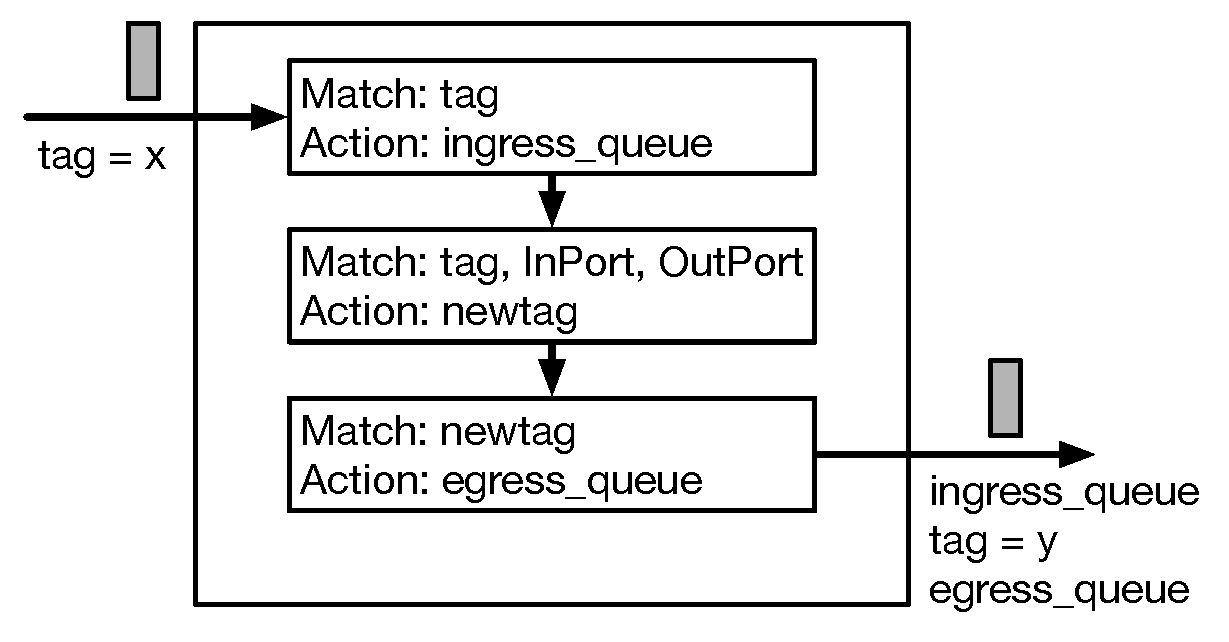
\includegraphics[width=0.4\textwidth] {figs/Tagger}
	\vspace{-1em}
	\caption{Tagger match-action rules}\label{fig:tagger}
	\vspace{-2em}
\end{figure}

\para {Match-Action rules:} \sysname{} needs to perform two operations at every
hop, i.e., {\em tag-based priority queueing} and {\em tag
rewriting}.  These two operations are implemented using a 3-step match-action
pipeline (Figure~\ref{fig:tagger}).  First, \sysname{} matches
the value of tags and classifies packets into ingress queues based. Second, 
\sysname{} matches (tag, InPort, OutPort) and rewrites the value of tag. 
The {\em third} step, wherein the packet is placed in an egress queue based on the
{\em new} tag value, is needed to ensure correct PFC operation, as described below.

\begin{figure}[t]
  \vspace{-3em}
 	\centering
 	\subfloat[short for lof][Ingress priority = egress priority  $\rightarrow$ packet drop.] {
 	%	\vspace{-3em}
 		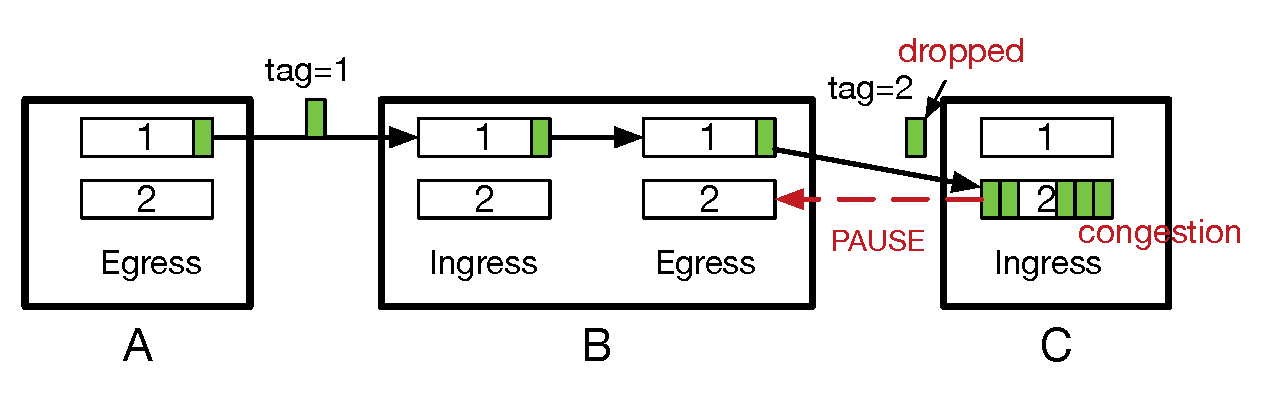
\includegraphics[width=0.4\textwidth] {figs/prioritydecoupling_1}
 	}
  \vspace{-1.2em}
  
 	\subfloat[short for lof][Ingress priority = 1, egress priority = 2 $\rightarrow$ no drop.]{
 		%\vspace{-3em}
 		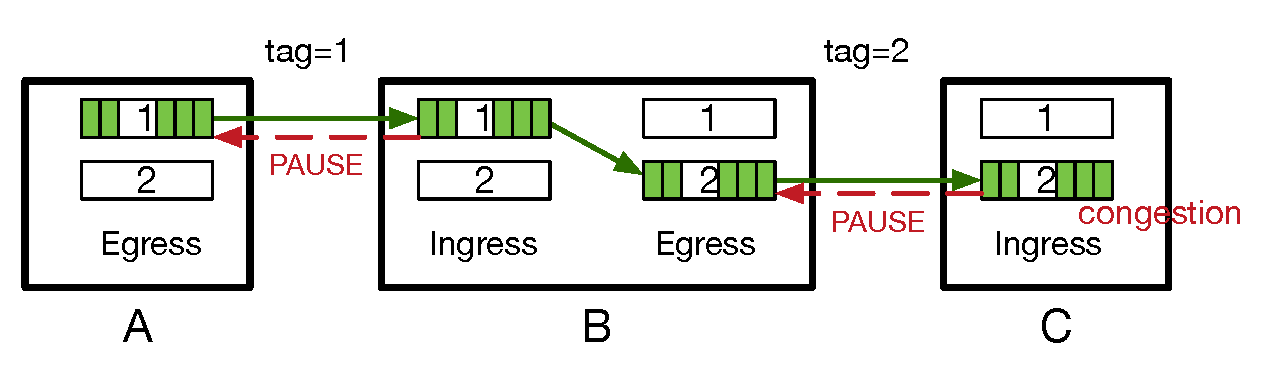
\includegraphics[width=0.4\textwidth] {figs/prioritydecoupling_2}
 	}
	 \vspace{-1em}
 	\caption{Decoupling ingress priority from egress priority at switch B is necessary for lossless priority transition.}\label{fig:prioritydecoupling}
	\vspace{-1em}
\end{figure}

\para{Handling priority transition:}
By default, a switch will enqueue a departing packet in the egress queue
of the same priority class as its ingress queue, as shown in Figure~\ref{fig:prioritydecoupling}(a).
In this example, Switch B is configured to 
perform priority transition for packets received from switch A and destined for switch C.
Packets exit egress queue 1 at switch B, but with priority 2. 
When ingress queue 2 of switch C becomes congested, the PFC PAUSE from switch C 
to switch B carries priority 2, and cannot pause the egress queue 1 of switch B.
This default behavior can lead to packet loss.

Therefore, we must map the packet to the egress queue
based on its new priority (Figure~\ref{fig:prioritydecoupling}(b)).  
This avoids packet loss, since the PFC from switch C
correctly pauses the queue on which the packet with the new tag would be
exiting.

\para{Rule compression:}  The match-action rules of \sysname{}
are implemented with TCAM. TCAM entries consist of {\em Pattern},
{\em Mask}, and {\em Result}. They refer to the pattern to be matched, the mask bits 
associated with the pattern and the action that occurs when a lookup hits the pattern, 
respectively.  One TCAM entry can have several Pattern-Mask pairs to match multiple packet header fields
simultaneously, e.g., an entry like (Pattern-1, Mask-1, Pattern-2, Mask-2, Result)
matches two fields simultaneously and fires only if both matches succeed.

\begin{figure}
	 
	\centering
	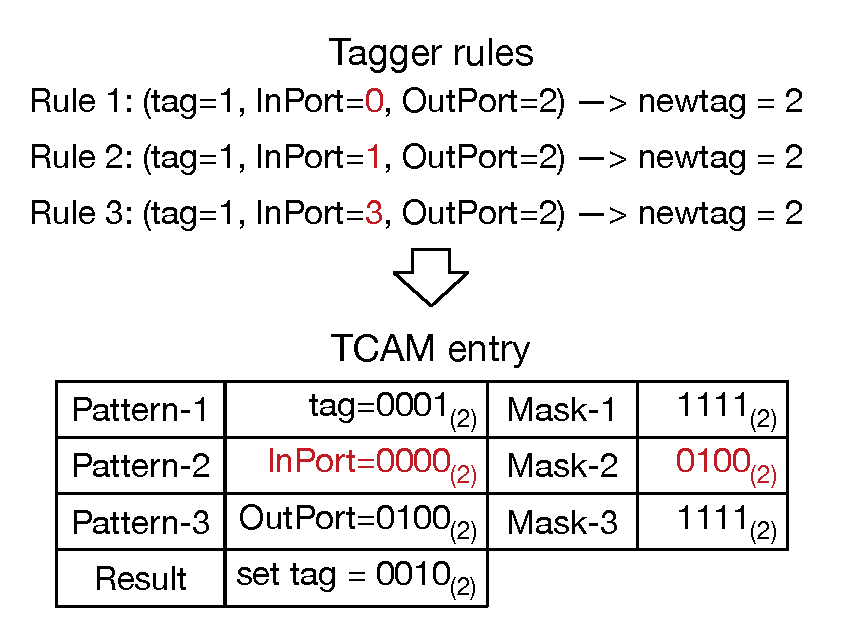
\includegraphics[width=0.37\textwidth] {figs/compression_with_bitmasking}
	\vspace{-1em}
	\caption{Rule compression with bit masking. Port numbers are bitmaps.
	The first bit from right represents port 0. The second bit represents port 1, and so on. }\label{fig:compression}
    \vspace{-1.5em}	
\end{figure}

Rules with the same Result can be compressed into one TCAM entry, if their
Patterns can be aggregated using bit masking. Consider the three
rules in Figure~\ref{fig:compression}. These rules are identical except the InPort
field in Pattern.

On commodity ASICs, port numbers in TCAM are bitmaps, not binary values. To match a single 
port, we can simply set the corresponding bit in the pattern to 1, and set the mask to all 1's. 
However, we may match multiple ports with one rule. We set the pattern to 
all 0's, and set the corresponding bits in the mask to 0. As shown in Figure~\ref{fig:compression},  
to match InPorts 0, 1 and 3, we set Pattern-2 to ``0000''  and Mask-2 to ``0100''. In this case, 
only the packet received from InPorts 0, 1 or 3 will match Pattern-2 after doing bit masking with Mask-2. 
Thus, the three rules are compressed into a single TCAM entry.

Recall from \S\ref{sec:generic} that without any compression, we need
$n(n-1)m(m-1)/2$ rules per switch. The number of rules can be
compressed to $nm(m-1)/2$ by aggregating InPorts.  The
result can be further improved by doing joint aggregation on tag, InPort and
OutPort.

\para{Broadcom implementation:} We implemented \sysname{} on commodity
switches based on Broadcom ASICs.  We use DSCP field in IP header as the tag.
The DSCP-based ingress priority queuing (step 1), ingress ACL and DSCP rewriting (step 2),
and ACL-based egress priority queuing (step 3) are well supported by the
commodity ASICs and do not require any ASIC changes. \shuihai{Everything is implemented using available and documented functionality.}

%Everything is implemented using publicly available and documented functionality.

%DSCP rewriting is supported by all commodity ASICs. DSCP-based priority
%queuing (step 1) is supported natively by all switch ASIC vendors. Step 2 uses
%ingress ACL rules to map (DSCP, InPort, OutPort) to new DSCP.

%Step 3 also uses ACLs, although it relies on certain details that are specific
%to Broadcom's match-action pipeline. We omit these gritty details for brevity.
%While the implementation of this step is Broadcom-specific, we believe that
%ASICs from other vendors can also support this functionality.

%%comment: this claim is not true, as brcm sdk is never public.
%%         
%We stress that none of the three steps require any changes to the switch ASIC,
%and everything is implemented using publicly available and documented
%functionality.

We considered using TTL instead of DSCP to tag packets, but TTL is automatically 
decremented by the forwarding pipeline, which complicates the rule structure.

